\chapter{Results}\label{chap:results}

\section{Example Figure}

Figures should be introduced in the text before they appear. As shown in \figref{fig:example}, Elliott Hall is used here as an example figure that you should replace with a final, accessible research figure.

\begin{figure}[p]
  \centering
  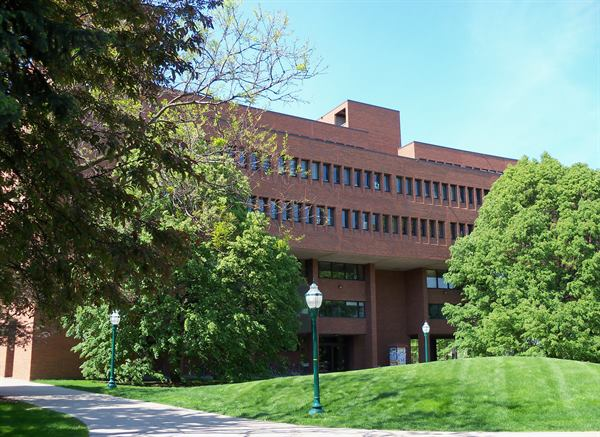
\includegraphics[width=\textwidth,height=0.62\textheight,keepaspectratio]{elliott-hall-cc-by-sa-3.0-template.jpg}
  \caption{Elliott Hall at the Minneapolis campus of the University of Minnesota. Photograph by AlexiusHoratius (2010), licensed CC BY-SA 3.0 via Wikimedia Commons. This image demonstrates a full-page figure layout. Replace it with a final research figure and a self-contained caption that defines all symbols, colors, error bars, and abbreviations needed for interpretation.}
  \label{fig:example}
  \addcontentsline{lof}{figure}{\protect\numberline{\thefigure.}Elliott Hall at the University of Minnesota}
\end{figure}

\section{Interpretation}

Report the result, then explain how it bears on the research question. Distinguish observed results from interpretation.
